\mySection{The Design of PyRollCall}
In this section, we present the use cases and the design of PyRollCall's architecture.
In the following context, a "user" refers to a "teacher" who wishes to perform roll calls
using PyRollCall, since the end user of this system is typically a teacher. In other words,
students are not the direct users of this system.
Figure~\ref{fig:use-case-diagram} shows the use case diagram of PyRollCall, whereas
Figure~\ref{fig:system-architecture} shows the system architecture of PyRollCall.


\subsection{Use Cases}
\vspace{0.5cm}

\setstretch{1.0}
\begin{itemize}
  \item Users can maintain the data of the courses and students they teach.
  \item Users can collect students' photos and generate their facial measurements.
  \item Users can start a roll call, recording students' attendace via FRT.
  \item Users can export the results of roll calls to files.
  \item Users should be able to keep their data the next time they use the system.
  \end{itemize}
\setstretch{\myContentLineSpacing}

\begin{figure}[!htb]
  \centering
  \vspace{1cm}
  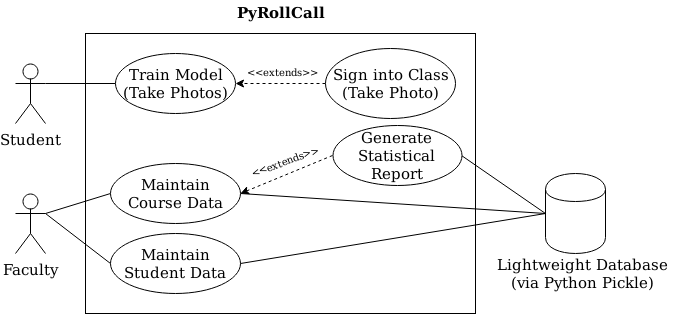
\includegraphics[width=\linewidth]{figures/use-case-diagram.png}
  \caption{Use Case Diagram}
  \label{fig:use-case-diagram}
  \vspace{1cm}
\end{figure}


\subsection{System Architecture}
The GUI front end is built with PyGTK, enabling users to easily have access
to the various functionalities in PyRollCall. Underneath the GUI, we use
OpenCV library to capture images via cameras, face\_recognition and dlib to
recognize faces of students, and pickle\footnote{pickle is a Python module
  which implements binary protocols to serialize and deserialize Python objects.}
to serialize and deserialize facial measurements (or facial embeddings).

\begin{figure}[!htb]
  \centering
  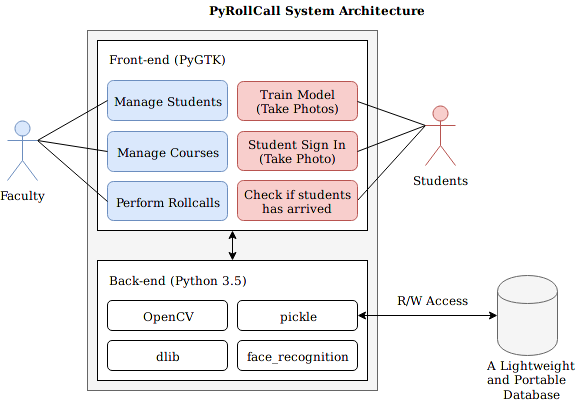
\includegraphics[width=\linewidth]{figures/system-architecture.png}
  \caption{System Architecture}
  \label{fig:system-architecture}
\end{figure}


\subsection{Implementation}
Text

\begin{algorithm}
\caption{A}
\label{alg:A}
\begin{algorithmic}
\STATE {set $r(t)=x(t)$}
\REPEAT
\STATE set $h(t)=r(t)$
\REPEAT
\STATE set $h(t)=r(t)$
\UNTIL{B}
\UNTIL{B}
\end{algorithmic}
\end{algorithm}
